\chapter{Discussion}
\label{chap:discussion}

This chapter first discusses certain problems with the experimental setup that could impact performance, before discussing the results from the experiments.
The last section will briefly mention recommendations for the future of de novo structure prediction from \ac{MS/MS}.

\section{Biases and overfitting}
\label{sec:overfitting}
 
A recurring problem for these string-based autoregressive models is the number of predictions that are identical to a label found in the training set.
When this occurs, it shows that a model is not able to achieve the task of predicting a de novo molecular representation from \ac{MS/MS}, but only repeats the data is has been trained with.
There are a few contributing factors to this overfitting problem with the setup used in this thesis.
Along with the problem of overfitting, there are some biases present in the experimental setup that are discussed in the following sections. 

\subsection{Duplicate training labels}
As mentioned in the paper from MassSpecGym \cite{bushuiev2024massspecgym}, the labeled dataset is a collection of the most qualitative annotated, open-source mass spectrometry datasets.
Even though a lot of filtering was performed after thorough quality control, the amount of duplicate molecules is significant.
Figure \ref{fig:duplicate_smiles} shows the amount of SMILES that have multiple occurrences in the training set. Notice the logarithmic y-axis for readability.
Even though 84\% of unique molecules have 10 occurrences or less, some molecules are noticeably more present, with one molecule being present 477 times in the training set.
This imbalance does not necessarily reflect the real-world imbalance of molecules as it is caused by the use of domain-focused datasets.
This causes the models to be trained with a bias towards these more frequent occurring molecules in the training set.
This imbalance is also present in the validation (and test) set, where the most frequently occurring molecule accounts for 2.7\% (out of the almost 20.000 entries) of the validation data.
Because of this imbalance, the models will be evaluated with a bias towards these more abundant molecules.
\begin{figure}[h]
    \centering
    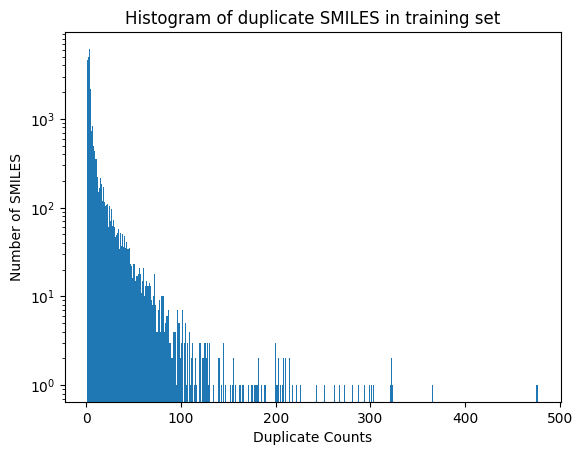
\includegraphics[width=0.6\textwidth]{figures/discussion/duplicate_smiles_training_set.png}
    \caption{distribution of duplicate SMILES in MassSpecGym's training set with a logarithmic scale}
    \label{fig:duplicate_smiles}
\end{figure}

\subsection{Exposure bias}

During training, a teacher forcing approach is used, where only the ground truth tokens are used to generate the next token iteratively.
At inference time, when the model is sampled, the model does not get this help and has to rely on its own previous (incorrect) predictions.
This is often referred to as exposure bias \cite{schmidt2019generalization}.
The previously discussed imbalance of the training set only makes this bias worse, by training on these frequently occurring token combinations.
This severely hinders the generalization of the model.
An example of this exposure bias can be clearly seen in the results from the hyperparameter gridsearch (figure \ref{fig:gridsearch_vs_paper}), where a model with a lower validation loss performed worse after sampling.
The loss has this teacher forced advantage, while the metrics calculated on the sampled predictions do not.
Because all models, trained in this thesis, are optimized for validation loss, it can be questioned if they have been overfit on these teacher forced training molecules.

\subsection{Evaluation metrics}
The two metrics that are used to evaluate a molecular prediction, Tanimoto similarity and \ac{MCES} distance, are somewhat flawed.
As explained in section \ref{sec:tan_sim}, the Tanimoto similarity uses molecular fingerprints that are unable to store all structural information.
When the predicted structure is converted to a molecular fingerprint, some structural information is lost.
The prediction will thus not be evaluated completely.
The \ac{MCES} distance on the other hand does evaluate the whole molecular structure, but can in some cases behave sub-optimal.
Looking at the formula in section \ref{sec:mces_dist}, when the evaluation molecules have few edges in their molecular graphs, a model could instead of finding the \acf{MCES}, just minimize the edges in its prediction.
In an extreme case, where the model only predicts nothing (e.g. empty SMILES, zero edges in the molecular graph), the MCES distance will be equal to the number of edges of the ground-truth molecular graph.
Figure \ref{fig:edges} shows the distribution of edges in the molecular graphs from the molecules in MassSpecGym's labeled dataset.
With an average number of edges of 37.5, a model that predicts empty SMILES would have an evaluated MCES distance of 37.5 using MassSpecGym.
While during training, the model does not have access to the MCES distance and will thus probability not reach this extreme case, it does question if some \ac{MCES} distances have a bias towards shorter predictions by this flaw.

\begin{figure}[H]
    \centering
    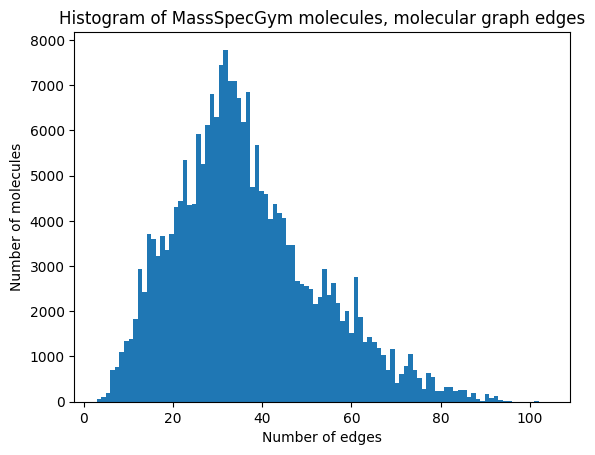
\includegraphics[width=0.6\textwidth]{figures/discussion/number_of_edges_massspecgym.png}
    \caption{distribution of number of edges from molecular graphs of molecules in MassSpecGym's labeled dataset SMILES}
    \label{fig:edges}
\end{figure}


Another limitation of both metrics is their inability to distinguish between de novo molecules and those seen during training.
This can cause problems when the models are not powerful enough to outperform overfitted models.
A model that, instead of predicting de novo molecules, would just rank the training molecules and return the most similar ones (similar to frequently used database lookup methods), could appear relatively good at predicting de novo molecules when only the \ac{MCES} distance and Tanimoto similarity are considered.
Only the number of novel molecules accurately shows if a model can generate de novo molecules.
Hence, to compare models, and decide which is better at predicting de novo molecules from \ac{MS/MS}, multiple metrics have to be considered.

\section{Experimental results}

Most of the results from the experiments in this thesis show no clear improvements over the methods used by the de novo models from MassSpecGym.
However, many conclusions can still be drawn from these results.
In hindsight, some experiments could still be improved upon by taking the results and discussion points from \ref{sec:overfitting} into account.
The following sections discuss the results and possible improvements for each experiment.

\subsection{Samplers benchmark}

The main conclusion from the samplers benchmark is that different samplers can perform better with different evaluation settings.
The deterministic samplers performed best with top-1 evaluation, showing their capability to predict valid molecules.
The probabilistic samplers, on the other hand, predicted more varying, sometimes invalid, molecules, which allowed them to outperform the deterministic samplers with a top-10 evaluation setting.

When predicting molecular structures from \ac{MS/MS}, randomness is not a desired property as there is only one correct molecular structure.
Even though multiple SMILES can represent the same molecular structure, overall we only want the correct atoms and bonds to be predicted.
A possible explanation for this phenomenon is that, on average, a bit of randomness could somewhat overcome the exposure bias from the overfitted model.

The beam search sampler's poor performance could also be linked to overfitting.
To verify this, the number of novel molecules should have been calculated.

In later experiments, it shows that the SMILES model used for this experiment was severely overfit on the training SMILES.
This experiment should in an ideal case also have to be repeated for a model that is able to predict more de novo molecules (e.g. SELFIES model).

\subsection{\ac{BPE} as pretraining}

Using \ac{BPE} increases the number of valid predictions at the cost of novel predictions. 
This conclusion is again confirmed by the molecular representations experiment in figure \ref{fig:representations}.
The main advantage is that by grouping multiple tokens as one, \ac{BPE} decreases the number of tokens the model has to predict.
When the model has less tokens to predict, it will make less mistakes, leading to more valid molecules.
In contrast, it will favour grouped tokens seen in the training data, and by having less tokens to predict, it will more often lead to predictions from the training set.
When using \ac{BPE}, the parameters of the algorithm should be tuned such that a balance between performance and minimal overfitting could be found.

While the results show that computing the \ac{BPE} on the 118M dataset did not improve the model's performance compared to the 4M dataset, even though it has almost 30 times more SMILES,
the quality of this dataset is considerably worse.
As explained in the MassSpecGym paper, the 118M dataset consists of all the available data from PubChem. 
No quality control was conducted for this dataset, which allows for an unrealistic distribution of chemical classes in the dataset.
An overrepresentation of one chemical class could severely influence the patterns found by the \ac{BPE} algorithm.
In contrast, the 4M dataset does have a controlled representation of multiple chemical classes.
This shows that quality is preferred over quantity.

\subsection{Augmentation}

Augmentation proved to be a difficult task for the SMILES de novo model.
Although the model noticeably overfits on the training data, augmentation has proven to be a great tool to combat overfitting \cite{shorten2019survey}.
Using other models, that experience less overfitting, would therefor probably not drastically change this experiment's results.

\subsubsection*{SMILES augmentation}

Figure \ref{fig:smiles_augm} shows that using SMILES synonyms as data augmentation does not improve the model's performance.
The number of novel molecules does increase when taking the number of valid molecules into account, as for the 5x synonyms model almost all valid predictions are novel predictions, compared to around 50\% of the not-augmented model.
A possible explanation for this worse performance is that the SMILES generation algorithm by RDkit (without random graph traversal) is deterministic.
It uses a canonicalization algorithm to generate this deterministic SMILES-string \cite{daylight_smiles_theory}.
Even though multiple SMILES can map to the same molecular structure, this algorithm will always be able to generate the same canonicalized SMILES-string from a molecular graph.
All SMILES labels in the MassSpecGym use this canonicalized format. 
By making the SMILES generation random, it could make training harder for the model.

A flaw in the setup of this experiment, is that all augmented models used the same tokenizer, for which \ac{BPE} was only computed on the canonicalized SMILES from the training set.
Only patterns from canonicalized SMILES were thus grouped in the vocabulary.
Random SMILES therefore used more tokens to describe their sequence, making it harder for the model.
This experiment also may have used too much augmentation, compared to the spectral augmentation experiment.
Too much augmentation will drown out the original data.
A model that was trained with e.g. 20\% augmented data may have improved performance.

Another way SMILES synonyms could combat overfitting would be to replace the duplicate SMILES from the training set by different synonyms.
Instead of keeping the original data as in the experiment, the model would not have these overrepresented SMILES, thus somewhat fixing the imbalance in the training set.
The drawback is, however, that the original canonicalized SMILES would be severely underrepresented and the bias towards these overrepresented molecules would still be present.

\subsubsection*{Spectral augmentation}

While figure \ref{fig:spectral_augm} shows no remarkable performance improvement, using a bit of augmented spectra does noticeably improve the number of valid and novel predictions.
Spectral augmentation thus proves to be useful to combat overfitting and increase generalization, when used moderately.

A possible improvement for this experiment would be to, instead of randomly augmenting 20\% of the spectra, try to fix the imbalance from the training set by augmenting the spectra of the underrepresented SMILES.

\subsection{Molecular representations benchmark}

From the results in figure \ref{fig:representations}, the SMILES model achieved the best MCES distance and Tanimoto similarity, while the SELFIES model seems to have the most novel predictions.
The modifications for autoregressive models implemented with DeepSMILES, do not seem to live up to expectations, performing worse than SMILES.
SELFIES is the only molecular representation from the benchmark where the number of novel prediction does not substantially drop when using \ac{BPE}.
This could be explained by the fact that some SELFIES tokens can have a different meaning in context of rings and branches. 
For example, a token that follows a branch token, only denotes the length of the branch, the original chemical meaning of the token does not matter for the prediction.
When this combination of branch and other token is stored with \ac{BPE}, the model cannot get confused by the original meaning of the second token.
The SELFIES alphabet is also much larger than the SMILES alphabet, which causes the sequence of tokens to be more diverse, reducing overfitting.
Because each SELFIES stores a lot of information, less tokens are needed to describe molecular structures, which remarkably does not seem to affect the number of novel predictions.

Overall, SELFIES seems to be the most robust molecular representation.
The reason SELFIES and DeepSMILES do not outperform the SMILES model could be due to multiple reasons.
(1) The optimal \ac{BPE} SMILES hyperparameters were used to train all the models with different molecular representations.
This could affect the performance compared to the SMILES model, as these hyperparameters might not be optimal for the other models.
In an ideal case, a hyperparameter search would have to be conducted to accurately compare the best performance for each model.
(2) The samplers for each evaluation setting were chosen based on the results from the sampler benchmark.
These samplers again used a \ac{BPE} SMILES model. Even though a temperature search was performed for the naive sampler.
The samplers used for each evaluation setting may not be optimal for models with different molecular representations.
The SMILES \ac{BPE} model hence had a noticeable advantage in this experiment, it is then only logical that it achieved the best performance.

The InchI representation is not suited for autoregressive prediction.
The idea for the multiple decoder model was to divide the prediction problem by predicting the layers from InchI separately.
Unfortunately, while the decoders did achieve at predicting valid predictions for their corresponding layer, the strict InchI structure needed them to exactly describe the same prediction.
They did not manage to synchronize their predictions which caused the combined InchI to be invalid.
To improve this model, these decoders should have a way to pass attention, to predict the same molecular structure.

\section{Future for de novo structure prediction}

The performance of the autoregressive models predicting string-based molecular representations, is very poor.
These models are not able to predict fully correct molecular structures from \ac{MS/MS}, as the complete structural accuracy on the validation and test set is close to zero percent.
Partly, this can be due to the imperfect training setup discussed in section \ref{sec:overfitting}, there might be too many biases for the model to overcome.
Some of these Biases however, can be fixed.
The data imbalance could be mitigated by annotating more \ac{MS/MS} spectra and filtering out overrepresented molecules.
Compared to other molecular datasets, MassSpecGym's labeled dataset is still relatively small.
While additional data is highly desirable, as in most machine learning contexts, obtaining it remains a significant challenge.
There are also a lot of methods that combat the exposure bias, e.g. scheduled sampling \cite{bengio2015scheduled} and professor forcing \cite{lamb2016professor}.
All these methods can not entirely mitigate the exposure bias problem as this remains an inherent problem when training autoregressive models.

It could be questioned if using these autoregressive models and string-based molecular representations are the best method for the de novo structure prediction.
While writing this Thesis, a new model, DiffMS \cite{bohde2025diffms}, was published that significantly changes the structure predicting pipeline.
Instead of using an autoregressive decoder to predict molecular structures, DiffMS uses a discrete graph diffusion model to, instead of using string-based representations, generate the molecular graph itself.
This model did succeed to predict 2.3\% of the test molecules for top-1 evaluation and 4.25\% for top-10 evaluation of MassSpecGym's test set.

Only recently has MassSpecGym introduced a standardized dataset to compare performance. De novo molecular structure prediction from \ac{MS/MS} is a very challenging task,
but even within a few months has DiffMS proven that the string-based autoregressive implementation is flawed.
Using graphical models to generate molecular structures seems to be the way forward instead of trying to use the methods from the natural language processing domain to predict string-based molecular representations.

\section*{Disclaimer, use of generative AI}

For this thesis, code generated by GPT-4o was used to speed up the design of the plots.
For the writing of this Thesis, GPT-4o helped rewriting certain sentences for clarity.